\chapter{設計と実装}
本性では,提案ツールを開発するときのアプローチを述べる.

\section{開発環境}
提案ツールの開発環境を下記に示す.

\begin{itemize}
    \item OS:macOS Big Sur 11.1
    \item プログラミング言語:Python 3.7
    \item 統合開発環境:PyCharm 2020.3.2
\end{itemize}

\section{提案ツールのアーキテクチャ}
\label{toolartchitecture}

\begin{figure}[H]
    \centering
    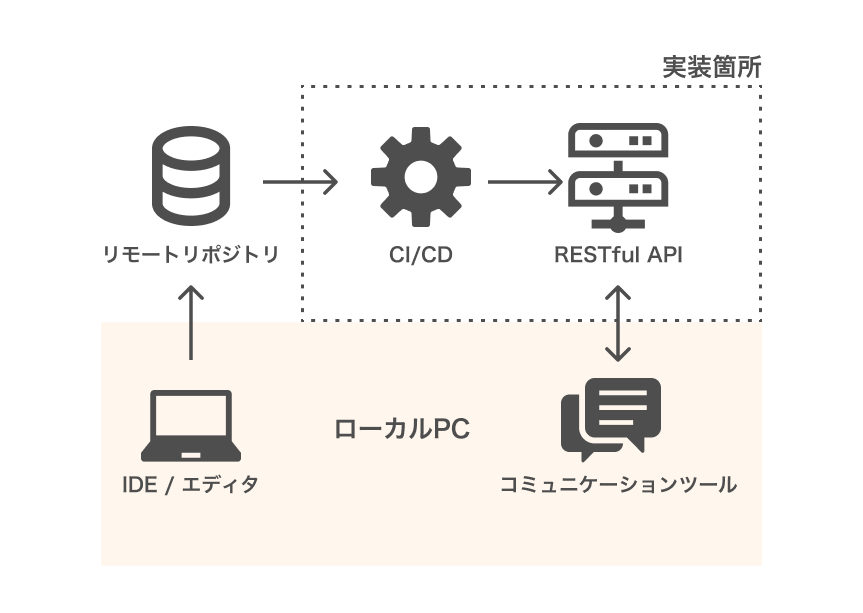
\includegraphics[width=12cm]{images/architecture.png}
    \caption{提案ツールのアーキテクチャ}
    \label{architecture}
\end{figure}

提案ツールのアーキテクチャを図\ref{architecture}に示す.
提案ツールは,既存のCI/CDツール上で動作することを想定しており,本研究ではCI/CDツールにGitHub Actionsを用いた.
また,CI/CDツール上で乖離の検知を行うが,できることが限られているため,同時に,Slackとのやりとりや,開発プロジェクトの状態の管理を行うことができるRESTful APIの開発も行った.
RESTful APIにはFastAPIを使用し,各種データの保持はJSONファイルにて管理を行っている.
また,RESTful APIは筆者のローカルPC上で動作させているが,HTTPSとして外部公開させることができるツールのngrokを使用しており,
Slack APIやCI/CDツール上で動作する提案ツールは,ローカルPC上で動作するRESTful APIを使用できるようになっている.

RESTful APIには,下記の機能をもたせているが,乖離検知の処理はすべてCI/CD上で動作するツールで行う.
\begin{itemize}
    \item 各機能のステータスを更新する機能
    \item Gitのコミットの差分量を追加する機能
    \item SlackのAPIを呼び出してメッセージを送受信する機能
\end{itemize}

Slackからに入力したコマンドをRESTful APIに反映させるための手順を下記にまとめる.
\begin{enumerate}
    \item Slackにコマンドを入力する
    \item Incoming Webhookより,SlackからRESTful APIに入力したコマンド内容がPOSTで送信される
    \item RESTful APIでは,受け取ったコマンドを解析し,適切な処理を行う
    \item 必要があれば,Slackにメッセージを送信する
\end{enumerate}

また,乖離検知を行い,検知した内容をSlackへと送信するための手順を下記にまとめる.
\begin{enumerate}
    \item GitHubへのプッシュを検知し,CI/CDツールが起動する
    \item CI/CD上で乖離検知を行うために,必要なデータをRESTful APIから取得する
    \item 取得したデータをもとに,乖離検知を行う
    \item 乖離検知をした場合,検知した内容を整形してメッセージとしてまとめ,RESTful APIにPOSTリクエストを行う
    \item RESTful APIからSlackにメッセージを送信する
\end{enumerate}

\section{提案ツールの使用方法}
開発者は,適切なタイミングで変更を記録するためにコミットを実行し,リモートリポジトリにプッシュすることを期待している.
\ref{toolartchitecture}節にまとめたとおり,提案ツールはリモートリポジトリにプッシュされたタイミングで,CI/CDツールが起動し,CI/CDツールの設定ファイルに定義されたコマンドに従って実行される.
そのため,提案ツールはGitHub Actionsを利用可能な状況ではローカルPCに専用の環境を構築せずに利用することができる.
ただし,提案ツールを利用するにあたっていくつか準備が必要であるため,それについてまとめる.
まず,CI/CDツール上で動作させるために,プロジェクトのディレクトリにtoolsディレクトリを作成し,そのディレクトリの中にPythonで作成された提案ツールを配置する.
CI/CDツールの設定ファイルには,プッシュ時に提案ツールを実行するように記述するだけでよい.
次に,SlackのAPIページより,提案ツールを登録する必要がある.
最後にRESTful APIの動作環境を用意する必要がある.例えばGCP(Google Cloud Platform)やHerokuなどのPaaS(Platform as aa Service)を利用することで,RESTful APIを動作する環境を用意することができる.
筆者が作成したRESTful APIをSaaSとして展開し,数多くのプロジェクトで利用することもできるが,セキュリティ上の懸念から各プロジェクトでRESTful APIを構築するのが望ましい.
いずれも,各Webサービスの登録手順に従って進めていくだけでよく,PaaSをよく理解していれば簡単に構築することができる.

\section{コミュニケーションツールで利用可能なコマンド}
milkでは,Slackのスラッシュコマンドを活用することで,各種パラメータの設定を行うことができるようになっている.
以下では,milkで使用可能なコマンドをまとめる.

\subsection*{/milk c1 doc [ file type ]}
ソースコード先行検知の機能において,開発プロジェクトで使用するSwaggerドキュメントのファイル形式を指定することができるコマンドである.
本コマンドは,開発プロジェクトの初期段階でSwaggerドキュメントのファイル形式を指定する場合や,開発プロジェクトの途中でファイル形式を変更したい場合に利用されることを想定している.

\subsection*{/milk c1 code [ file type ]}
ソースコード先行検知の機能において,開発プロジェクトで使用するプログラミング言語を指定することができるコマンドである.
現在では,プログラミング言語にPythonのみを指定可能である.

\subsection*{/milk c1 param}
ソースコード先行検知の機能において,現在設定しているSwaggerドキュメントの拡張子および使用しているプログラミング言語の拡張子を確認することができるコマンドである.

\subsection*{/milk c2 set [ days ]}
一定時間経過後のリマインダーの機能において,ドキュメントが更新されずソースコードのみが更新されている場合に,ドキュメントを追加・修正するためのリマインダーを行う間隔を指定することができるコマンドである.

\subsection*{/milk c2 param}
一定時間経過後のリマインダーの機能において,現在設定しているリマインダーを行う間隔を確認することができるコマンドである.

\subsection*{/milk c3 set [ version file ]}
リリース時ドキュメント更新有無の検知の機能において,バージョンを扱うファイルを指定することができるコマンドである.
例えば,Pythonではsetup.pyと呼ばれるファイルにソフトウェアのバージョンを記述している.
現在では,バージョンを扱うファイルにsetup.pyのみを指定可能である.

\subsection*{/milk c4 set [ number ]}
ソースコード変更量の検知の機能において,ドキュメントが更新されずソースコードのみが更新されている場合に,ソースコードの追加・削除・修正が行われた行数を指定することができるコマンドである.
指定した行数を超過してソースコードのみを記述し続けたときに通知がでる.

\subsection*{/milk c4 param}
ソースコード変更量の検知の機能において,現在設定している変更量を確認することができるコマンドである.
